\documentclass[11pt]{article}

\usepackage[spanish]{babel}
\usepackage[margin=1in]{geometry}
\usepackage{amsmath, amssymb, amsfonts}
\usepackage{graphicx}
\usepackage{float}
\usepackage{booktabs}
\usepackage{enumitem}
\usepackage{tcolorbox}
\usepackage{hyperref}
\usepackage{listings}
\usepackage{xcolor}
\usepackage{parskip}
\usepackage{pgfplots}
\usepackage{csquotes}
\usepackage[backend=biber,style=numeric,sorting=none]{biblatex}
\addbibresource{referencias.bib}

\usetikzlibrary{arrows.meta}
\pgfplotsset{compat=1.18}

\lstset{
  language=Python,
  basicstyle=\ttfamily\footnotesize,
  breaklines=true,
  columns=flexible,
  keepspaces=true,
  commentstyle=\color{gray}\itshape,
  keywordstyle=\color{blue!70!black}\bfseries,
  stringstyle=\color{green!40!black},
  frame=L,
  xleftmargin=2em,
  showstringspaces=false,
  tabsize=4
}

\setlist{itemsep=2pt, topsep=4pt}

\title{\textbf{Laboratorio 9: Respuestas} \vspace{1em}\\
  Deep Learning y Sistemas Inteligentes - CC3092}
\author{José Antonio Mérida Castejón}
\date{\today}

\begin{document}
\decimalpoint

\maketitle

\begin{tcolorbox}[colback=gray!8, colframe=gray!50, boxrule=0.5pt]
\textbf{Nota:} este informe fue generado con IA (Claude Code) a partir del notebook \texttt{Notebook.ipynb}, transcribiendo sus respuestas, tablas y figuras. El detalle del uso de IA está en \texttt{AI.md}.
\end{tcolorbox}

El código, las salidas y las gráficas de todos los tasks ya están en el notebook \texttt{Notebook.ipynb}; este documento contiene las respuestas a cada task. Semilla fija: \texttt{SEED = 42} (Python, NumPy y PyTorch/CUDA).

% =====================================================================
\section*{Task 1 --- Autoencoder variacional}

\subsection*{Task 1.1 --- Datos}
Fashion-MNIST escalado a $[0,1]$, últimos 5\,000 ejemplos de train como validación (train: 55\,000, val: 5\,000). Configuración: \texttt{batch\_size = 128}, \texttt{latent\_dim = 2}, \texttt{epochs = 20}, \texttt{lr = 1e-3}, \texttt{beta\_values = [0.1, 1.0, 10.0]}.

\subsection*{Task 1.2 --- Modelo y pérdida}
Funciones implementadas:
\begin{itemize}
  \item \texttt{reparameterize}: $z=\mu+\sigma\odot\epsilon$
  \item \texttt{kl\_divergence}: KL cerrada entre $\mathcal N(\mu,\mathrm{diag}(\sigma^2))$ y $\mathcal N(0,I)$, sumada sobre dimensiones latentes $\rightarrow$ un valor \textbf{por imagen}
  \item \texttt{vae\_loss}: $\|x-\hat x\|^2$ (suma sobre 784 píxeles) $+\ \beta D_{KL}$
\end{itemize}

\textbf{Arquitectura:} VAE completamente conectado, \texttt{latent\_dim = 2}.
\begin{itemize}
  \item \textbf{Encoder:} Flatten $\rightarrow$ 784$\rightarrow$512 $\rightarrow$ ReLU $\rightarrow$ 512$\rightarrow$256 $\rightarrow$ ReLU
  \item \textbf{Heads:} \texttt{fc\_mu} y \texttt{fc\_lv}, cada uno 256$\rightarrow$2 ($\mu$ y $\log\sigma^2$)
  \item \textbf{Decoder:} 2$\rightarrow$256 $\rightarrow$ ReLU $\rightarrow$ 256$\rightarrow$512 $\rightarrow$ ReLU $\rightarrow$ 512$\rightarrow$784 $\rightarrow$ Sigmoid $\rightarrow$ (1, 28, 28)
\end{itemize}

\begin{figure}[H]
\centering
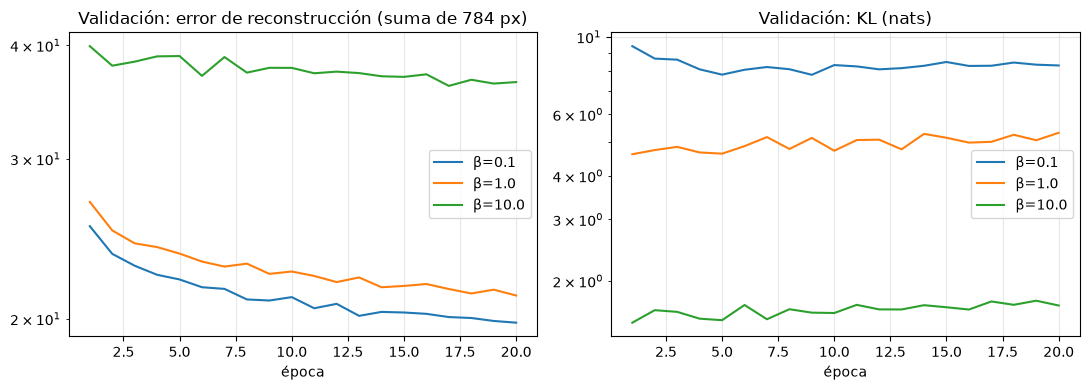
\includegraphics[width=0.95\textwidth]{figs/vae_curvas.png}
\caption{Curvas de validación del error de reconstrucción y de la KL por época, para cada $\beta$.}
\end{figure}

\subsection*{Task 1.3 --- Figuras}

\textbf{(a)} Dispersión de $\mu$ en validación, coloreada por clase.
\begin{figure}[H]
\centering
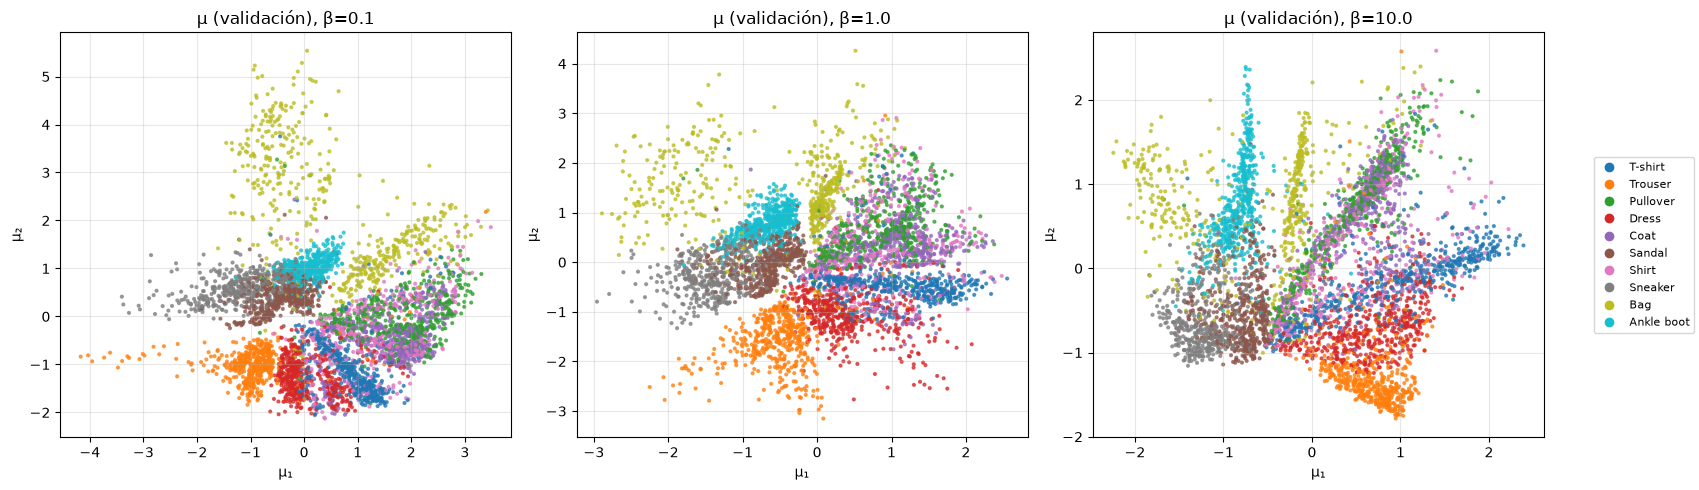
\includegraphics[width=\textwidth]{figs/vae_scatter.png}
\end{figure}

\textbf{(b)} Cuadrícula $15\times15$ de $z\in[-3,3]^2$ decodificada, $\beta=1$ (la fila superior corresponde a $z_2=+3$).
\begin{figure}[H]
\centering
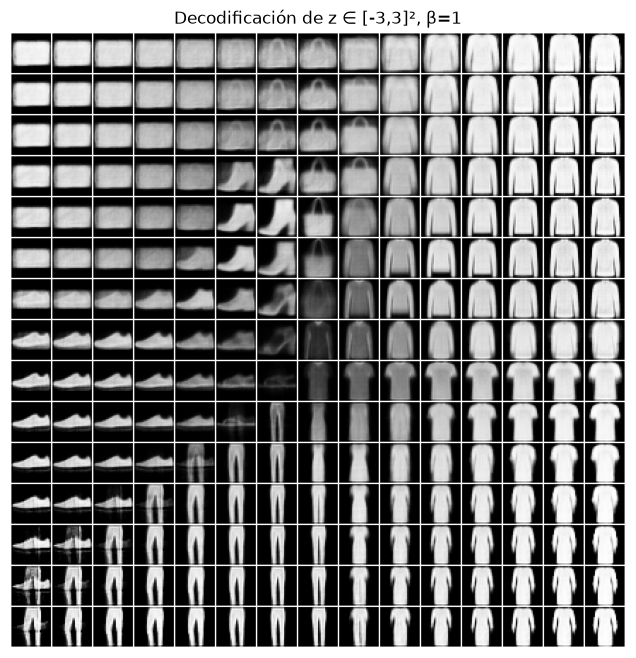
\includegraphics[width=0.6\textwidth]{figs/vae_grid.png}
\end{figure}

\textbf{(c)} 64 imágenes generadas con $z\sim\mathcal N(0,I)$ por cada $\beta$.
\begin{figure}[H]
\centering
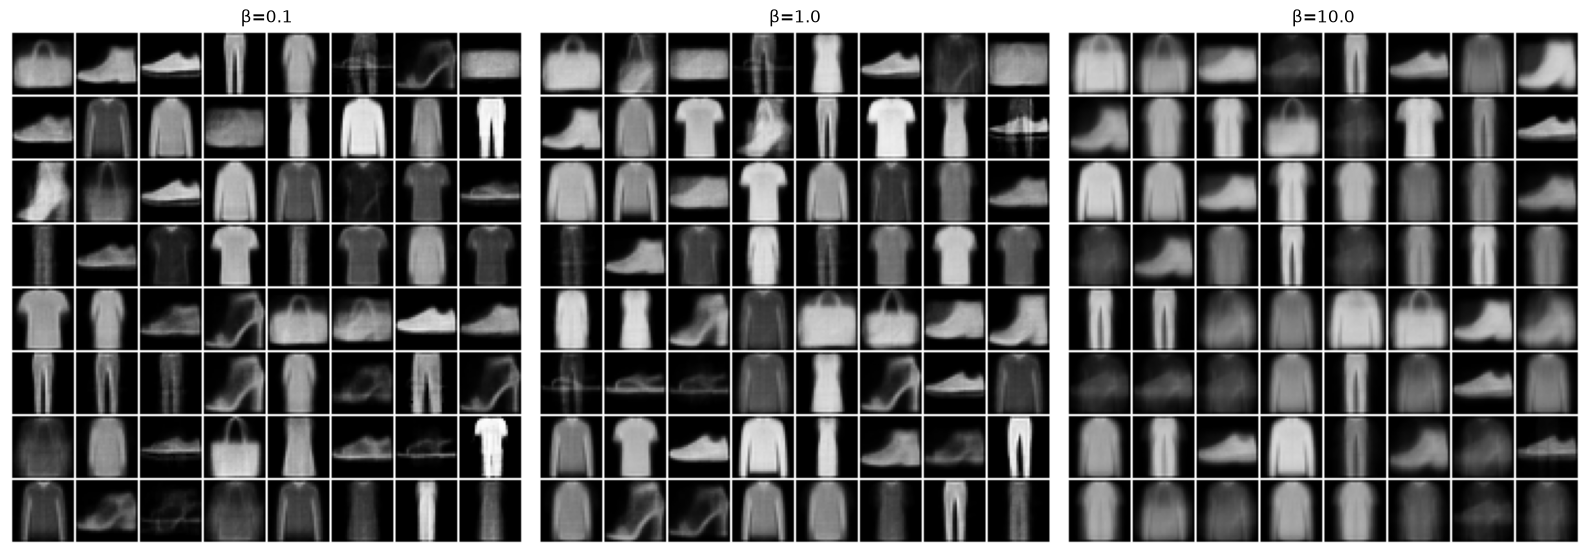
\includegraphics[width=\textwidth]{figs/vae_samples.png}
\end{figure}

\textbf{(d)} Interpolación entre dos imágenes de validación de clases distintas (8 puntos intermedios), $\beta=1$: píxeles vs.\ espacio latente (sobre $\mu$).
\begin{figure}[H]
\centering
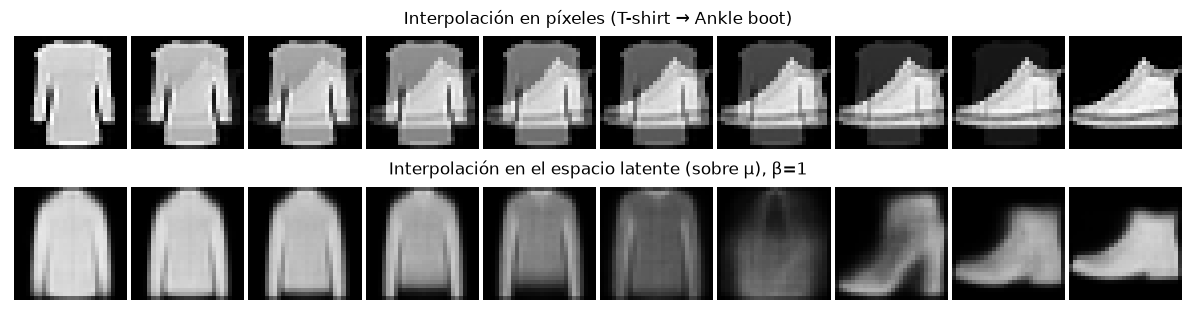
\includegraphics[width=\textwidth]{figs/vae_interp.png}
\end{figure}

\subsection*{Task 1.4 --- Análisis}

\subsubsection*{(a) Reconstrucción y KL finales de validación, KL en bits vs.\ $\log_2 10\approx3.32$ bits}
\begin{table}[H]
\centering
\begin{tabular}{cccc}
\toprule
$\beta$ & recon (val) & KL nats (val) & KL bits (val) \\
\midrule
0.1 & 19.808 & 8.277 & 11.941 \\
1.0 & 21.247 & 5.308 & 7.658 \\
10.0 & 36.765 & 1.700 & 2.452 \\
\bottomrule
\end{tabular}
\end{table}

Al subir $\beta$ la reconstrucción empeora y el KL baja: recon 19.8 $\rightarrow$ 21.2 $\rightarrow$ 36.8 y KL 8.28 $\rightarrow$ 5.31 $\rightarrow$ 1.70 nats (11.9 $\rightarrow$ 7.7 $\rightarrow$ 2.5 bits) para $\beta$ = 0.1, 1, 10. Con $\beta$ pequeño el modelo prioriza reconstruir y se aleja del prior; con $\beta$ grande el término KL domina y el código latente transmite menos información.

Para $\beta$ = 0.1 y $\beta$ = 1 el KL (11.9 y 7.7 bits) supera $\log_2 10 \approx 3.32$ bits, así que hay capacidad de sobra para codificar la clase. Para $\beta$ = 10 el KL es 2.45 bits $<$ 3.32, el código no alcanza para identificar la clase de una imagen de forma fiable y además esos bits deben describir también la forma y el estilo. Esto coincide con el diagrama de dispersión de $\beta$ = 10: las clases de forma muy distinta (Trouser, Bag, Ankle boot, Sneaker/Sandal) ocupan regiones propias, pero T-shirt, Pullover, Coat, Shirt y Dress se superponen en una sola zona. Es decir, el código distingue solo $\sim$5--6 grupos ($2^{2.45} \approx 5.5$) en lugar de 10 clases

\subsubsection*{(b) KL por Monte Carlo vs.\ KL cerrada}
KL por Monte Carlo ($10^5$ muestras de $q(z|x)$, promedio de $\log q(z)-\log p(z)$) vs.\ KL cerrada, $\beta=1$, una imagen de validación.

Para una imagen de validación, con el modelo $\beta=1$ ($\mu=[1.761,\,0.214]$, $\sigma=[0.164,\,0.079]$):
\begin{table}[H]
\centering
\begin{tabular}{lc}
\toprule
Método & KL (nats) \\
\midrule
Forma cerrada & 4.93679 \\
Monte Carlo ($10^5$ muestras) & 4.93691 $\pm$ 0.00324 \\
\bottomrule
\end{tabular}
\end{table}

\textbf{Error relativo:} $2.4\times10^{-5}$ (diferencia absoluta $\approx 1.2\times10^{-4}$).

\textbf{¿Es compatible con la variabilidad Monte Carlo?} Sí. El error estándar del estimador es $\text{SE}=s/\sqrt{N}\approx0.0032$, y la diferencia observada es solo $0.04$ SE. Una fluctuación típica sería de alrededor de 1 SE, así que la diferencia está muy dentro de lo esperado.

Esto confirma que la fórmula cerrada
\[D_{KL}=\tfrac12\sum_j\left(\mu_j^2+\sigma_j^2-1-\log\sigma_j^2\right)\]
está bien implementada.

\subsubsection*{(c) Región del espacio latente no reconocible; punto medio de las interpolaciones}
Con $\beta=1$ las imágenes de las esquinas de la cuadrícula siguen siendo reconocibles. Los zapatos a la izquierda, pantalones abajo a la izquierda y prendas de manga larga a la derecha. La región no reconocible está cerca del origen, en la frontera entre las zonas de zapato (Sneaker/Ankle boot), pantalón y prendas superiores (aprox. $z_1\in[-1,0]$, $z_2\in[-1,0.5]$). Ahí el decoder produce imágenes oscuras y tenues, sin forma de ninguna clase.

El término KL empuja los posteriores $q(z|x)$ hacia $\mathcal N(0,I)$, de modo que las clases quedan juntas y solapadas alrededor del origen. En una frontera, el mismo $z$ puede venir de imágenes de clases distintas y como la pérdida es un error cuadrático, el decoder aprende a producir el promedio de ellas. Con $\beta$ más grande el overlap sería mayor y más zonas se verían así; con $\beta$ pequeño habría huecos con menos datos donde el decoder se entrena poco.

En píxeles, el punto medio es una superposición lineal de las dos imágenes, se ven a la vez las mangas de la camiseta y la silueta de la bota, cada una al 50\% de intensidad. Esto claramente no es una imagen plausible de ninguna clase. En el espacio latente, el punto medio $\mu=\tfrac12(\mu_a+\mu_b)$ se decodifica con una red no lineal, así que no hay superposición. La secuencia se mantiene como una prenda de manga larga que se va desvaneciendo, pasa por una mancha oscura y borrosa (el punto medio cae en la frontera entre clases, la región descrita arriba) y luego cambia de golpe a una bota. Difieren porque la interpolación en píxeles es lineal en el espacio de imagen, mientras que la latente es lineal en $z$ pero pasa por el decoder, que mapea la zona entre clases a su ``imagen promedio'' borrosa y no a una mezcla de ambas.

\subsubsection*{(d) Nitidez y relación con $\sigma_x^2$}
\textbf{Nitidez} (media de $|x_{j+1}-x_j|$, 1\,000 imágenes cada una):
\begin{table}[H]
\centering
\begin{tabular}{cccc}
\toprule
Real & VAE $\beta=0.1$ & VAE $\beta=1$ & VAE $\beta=10$ \\
\midrule
0.0891 & 0.0446 & 0.0501 & 0.0439 \\
\bottomrule
\end{tabular}
\end{table}

Las muestras del VAE tienen alrededor de la mitad de la nitidez de las imágenes reales.

\textbf{Relación con $\sigma_x^2$.} Con decoder gaussiano, el negativo del ELBO es proporcional a $\|x-\hat x\|^2 + 2\sigma_x^2 D_{KL}$. Mi pérdida es $\mathcal L_\beta=\|x-\hat x\|^2+\beta D_{KL}$, así que $2\sigma_x^2=\beta$, es decir, $\sigma_x^2=\beta/2$.

\textbf{Por qué salen borrosas.} Con $\beta=1$, el modelo supone un ruido por píxel de $\sigma_x\approx0.7$, enorme para imágenes en $[0,1]$. Por eso casi no se penaliza producir imágenes suavizadas. Además, al entrenar con error cuadrático, el decoder aprende la media $\mathbb E[x\mid z]$. Esa media promedia los bordes y texturas posibles, y el resultado es borroso. Esto explica que todas las muestras pierdan cerca de la mitad de la nitidez.

La diferencia entre valores de $\beta$ es pequeña y no monótona (0.044--0.050, una sola semilla), así que no permite sacar conclusiones sobre el efecto de $\beta$.

% =====================================================================
\section*{Task 2 --- Proceso forward de difusión}

\subsection*{Task 2.1 --- Calendario y fórmula cerrada}
Datos escalados a $[-1,1]$, con $T=1000$, $\beta_{\text{start}}=10^{-4}$ y $\beta_{\text{end}}=0.02$. Convención de índices: los tensores del calendario tienen longitud $T+1$ y se indexan \textbf{directamente por $t\in\{1,\dots,T\}$}; la posición 0 es un relleno ($\beta_0=0,\ \alpha_0=\bar\alpha_0=1$, es decir $x_0$). La fórmula cerrada implementada es $x_t=\sqrt{\bar\alpha_t}\,x_0+\sqrt{1-\bar\alpha_t}\,\epsilon$. Para el calendario lineal, $\bar\alpha_T = 4.0358\times10^{-5}$.

\subsection*{Task 2.2 --- Verificación empírica de la fórmula cerrada}
5\,000 copias de una imagen $x_0$, 300 pasos $x_s=\sqrt{\alpha_s}x_{s-1}+\sqrt{\beta_s}\epsilon_s$ con ruido independiente, y comparación contra $\sqrt{\bar\alpha_{300}}x_0$ y $1-\bar\alpha_{300}$.

\begin{table}[H]
\centering
\begin{tabular}{lc}
\toprule
Cantidad & Valor \\
\midrule
$\bar\alpha_{300}$ & 0.39642 \\
Varianza teórica $1-\bar\alpha_{300}$ & 0.60358 \\
Error máximo $|\text{media}_{\text{emp}}-\text{media}_{\text{teo}}|$ & 0.03352 \\
Error estándar esperado $\sigma/\sqrt N$ & 0.01099 \\
Varianza empírica media & 0.60376 \\
$|\text{var}_{\text{emp}}-\text{var}_{\text{teo}}|$ medio & 0.00936 \\
\bottomrule
\end{tabular}
\end{table}

\textbf{Sí, es compatible.} Cada píxel de la media empírica promedia $N=5000$ muestras con varianza $1-\bar\alpha_{300}=0.60358$, así que
\[\text{SE}=\sqrt{0.60358/5000}=0.011.\]
El error máximo observado es $0.0335\approx3\,\text{SE}$. Como es el máximo sobre 784 píxeles, eso es lo esperado: el máximo de 784 normales suele estar cerca de $3.2\,\text{SE}$.

La varianza también coincide: $0.60376$ empírica frente a $0.60358$ teórica, con un error medio de $\approx0.8\,\text{SE}$, que es justo lo esperado.

\subsection*{Task 2.3 --- Visualización y SNR}

\textbf{(a)} $x_t$ para $t\in\{1,50,100,250,500,750,1000\}$ (Trouser, Sandal, Ankle boot).
\begin{figure}[H]
\centering
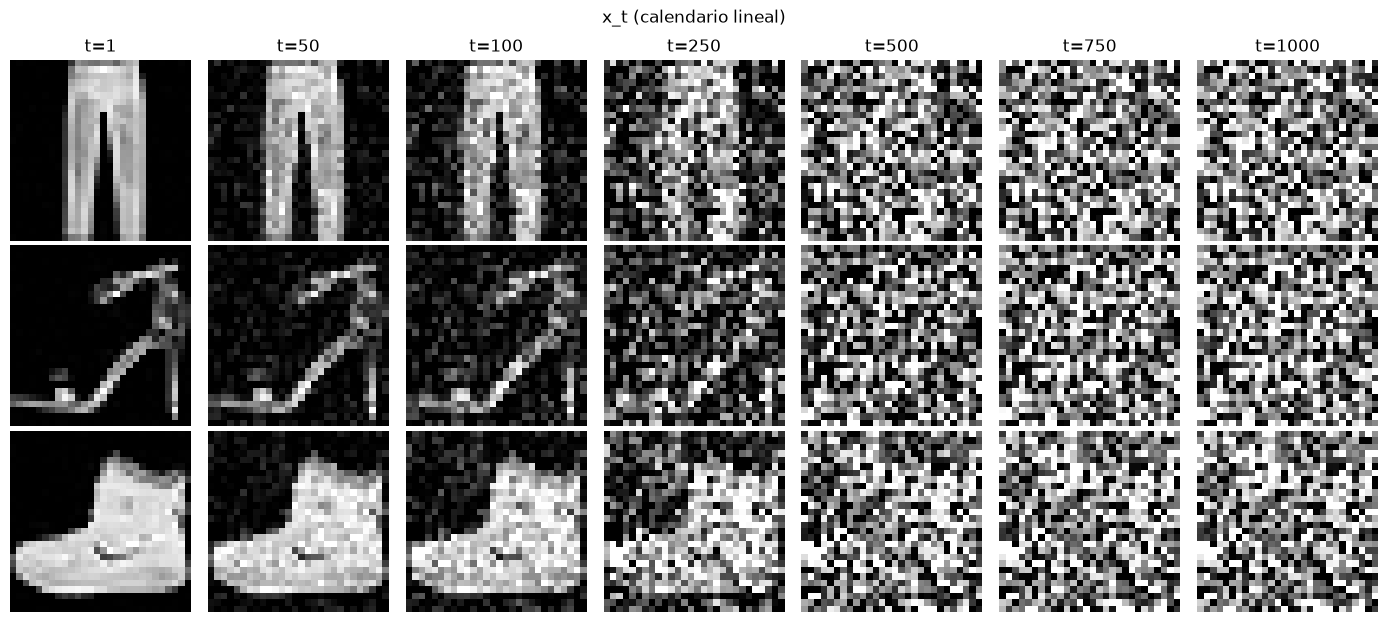
\includegraphics[width=0.9\textwidth]{figs/diff_xt.png}
\end{figure}

\textbf{(b)} $\bar\alpha_t$ y $\mathrm{SNR}(t)=\bar\alpha_t/(1-\bar\alpha_t)$ (escala logarítmica).
\begin{figure}[H]
\centering
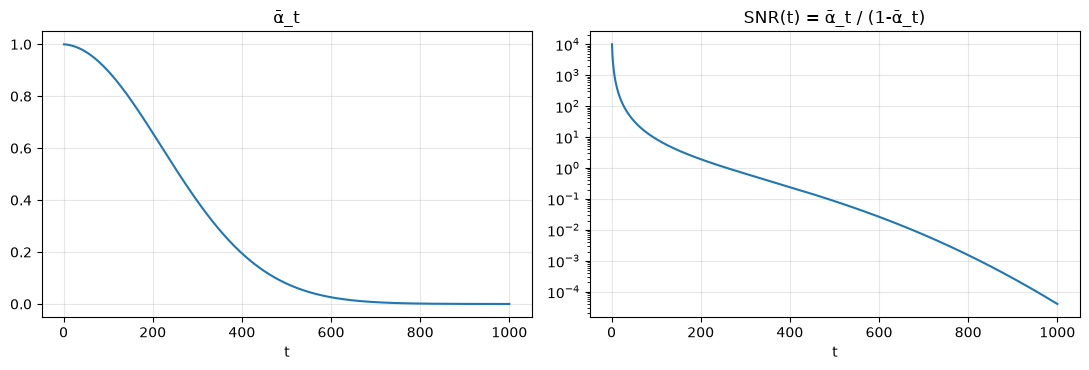
\includegraphics[width=0.9\textwidth]{figs/diff_snr.png}
\end{figure}

\textbf{(c)}
\begin{itemize}
  \item Primer $t$ con $\mathrm{SNR}(t)<1$: $\mathbf{t=260}$
  \item Primer $t$ con $\bar\alpha_t<0.01$: $\mathbf{t=674}$
\end{itemize}

\subsection*{Task 2.4 --- Segundo calendario}
Claude fue el encargado de implementar el segundo calendario, se le indicó que tomara alguno popular, lo citara e implementara con alguna modificación.

Calendario coseno de Nichol \& Dhariwal (2021)~\cite{nichol2021}, $\bar\alpha_t = f(t)/f(0)$, $f(t) = \cos^2\!\left(\frac{t/T + s}{1+s}\cdot\frac{\pi}{2}\right)$, $s = 0.008$, con $\beta_t = 1 - \bar\alpha_t/\bar\alpha_{t-1}$ recortado a $[10^{-5}, 0.999]$. Cumple $\bar\alpha_T < 10^{-3}$ y $\beta_t\in(0,1)$.

\begin{figure}[H]
\centering
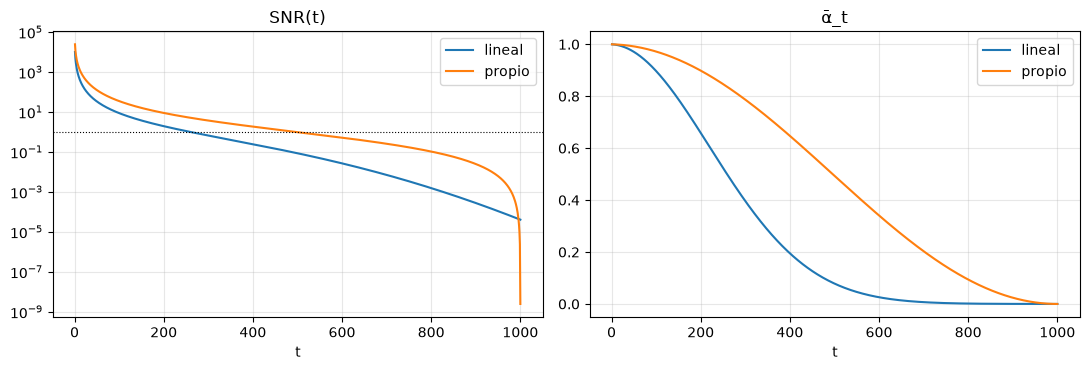
\includegraphics[width=0.9\textwidth]{figs/sched_cmp.png}
\end{figure}

\begin{table}[H]
\centering
\begin{tabular}{lcc}
\toprule
Calendario & $\bar\alpha_T$ & Primer $t$ con SNR $<1$ \\
\midrule
Lineal & $4.0358\times10^{-5}$ & 260 \\
Propio (coseno) & $2.4288\times10^{-9}$ & 497 \\
\bottomrule
\end{tabular}
\end{table}

\subsection*{Task 2.5 --- Análisis}

\subsubsection*{(a) Aproximación $\log\bar\alpha_T\approx-\sum_t\beta_t-\tfrac12\sum_t\beta_t^2$}
Con $\beta_t$ lineal de $10^{-4}$ a $0.02$ y $T=1000$:
\[\sum_t\beta_t=\frac{T(\beta_1+\beta_T)}{2}=10.05,\qquad \sum_t\beta_t^2\approx\frac{T}{3}\left(\beta_1^2+\beta_1\beta_T+\beta_T^2\right)=0.1340.\]
\[\log\bar\alpha_T\approx-10.05-\tfrac12(0.1340)=-10.117\ \Rightarrow\ \bar\alpha_T\approx4.04\times10^{-5}.\]
El valor exacto del código es $4.0358\times10^{-5}$ (diferencia de $\approx0.07\%$, debida al término de tercer orden omitido). Las sumas calculadas en la celda coinciden con las hechas a mano.

\subsubsection*{(b) Pasos con $\mathrm{SNR}\in[0.01,100]$ por calendario}
\begin{table}[H]
\centering
\begin{tabular}{lccc}
\toprule
Calendario & SNR $\in[0.01,100]$ & SNR $<0.01$ & SNR $>100$ \\
\midrule
Lineal & 647 & 326 & 27 \\
Coseno & 880 & 64 & 56 \\
\bottomrule
\end{tabular}
\end{table}

\begin{itemize}
  \item \textbf{SNR $<0.01$:} $x_t\approx\epsilon$, así que predecir $\epsilon$ es trivial y aporta poco gradiente.
  \item \textbf{SNR $>100$:} $x_t\approx x_0$, así que aislar el ruido es muy difícil (es el intervalo con mayor MSE en la Task 3.2). Son pocos pasos.
  \item \textbf{SNR $\in[0.01,100]$:} señal y ruido son comparables, y la tarea es informativa.
\end{itemize}

El coseno es más eficiente: el 88\% de sus pasos están en el rango útil, frente al 65\% del lineal, y desperdicia muchos menos en ruido puro (64 frente a 326).

\subsubsection*{(c) $\mathrm{Var}(x_t)=\bar\alpha_t\mathrm{Var}(x_0)+(1-\bar\alpha_t)$}
Como $\epsilon$ es independiente de $x_0$ y $\mathrm{Var}(\epsilon)=1$:
\[\mathrm{Var}(x_t)=\bar\alpha_t\,\mathrm{Var}(x_0)+(1-\bar\alpha_t).\]
Verificación con $\mathrm{Var}(x_0)=0.49826$:
\begin{table}[H]
\centering
\begin{tabular}{ccc}
\toprule
$t$ & Empírica & Predicción \\
\midrule
1 & 0.4983 & 0.4983 \\
250 & 0.7369 & 0.7370 \\
500 & 0.9604 & 0.9606 \\
1000 & 1.0003 & 1.0000 \\
\bottomrule
\end{tabular}
\end{table}

Como $\bar\alpha_T\approx0$, se tiene $\mathrm{Var}(x_T)\approx1$ sin importar los datos. Esto es necesario porque el muestreo empieza en $x_T\sim\mathcal N(0,I)$. Si el proceso forward terminara en otra distribución, habría un desajuste entre entrenamiento y generación.

% =====================================================================
\section*{Task 3 --- Difusión condicional y guía sin clasificador}

\subsection*{Task 3.1 --- U-Net condicional}
Entrada $x_t$ \texttt{(B,1,28,28)}, instante $t$ \texttt{(B,)} (valores $1..T$) y clase $c$ \texttt{(B,)} en $\{0,\dots,10\}$ (10 = condición nula). Dos niveles (28$\times$28 con 32 canales; 14$\times$14 con 64), cuello de botella 14$\times$14, subida con \emph{skip connections} concatenadas, convolución final a 1 canal. Embedding sinusoidal de $t$ (misma fórmula de la Semana 6) + MLP, \texttt{nn.Embedding(11, d)} para la clase; la suma se inyecta con \emph{broadcasting} en cada bloque.

Esta sección fue implementada utilizando IA, detallado en \texttt{AI.md}.

La U-Net condicional tiene \textbf{364,257 parámetros} entrenables.

\subsection*{Task 3.2 --- Entrenamiento}
Por iteración: $t\sim U\{1,\dots,T\}$, $\epsilon\sim\mathcal N(0,I)$, $x_t$ con \texttt{q\_sample}, clase $\rightarrow$ 10 con probabilidad \texttt{p\_uncond}, MSE entre $\epsilon$ y la predicción (\texttt{epochs = 30}, \texttt{batch\_size = 128}, \texttt{lr = 2e-4}, \texttt{p\_uncond = 0.1}).

\begin{figure}[H]
\centering
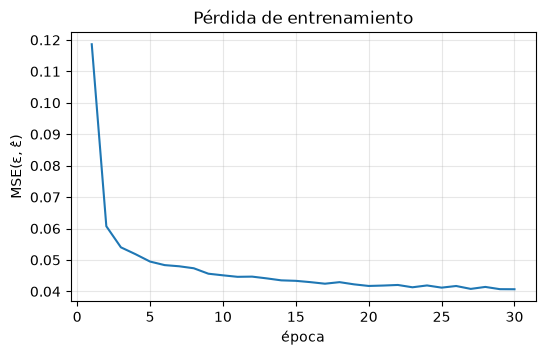
\includegraphics[width=0.55\textwidth]{figs/diff_train_loss.png}
\caption{Pérdida de entrenamiento por época.}
\end{figure}

\begin{figure}[H]
\centering
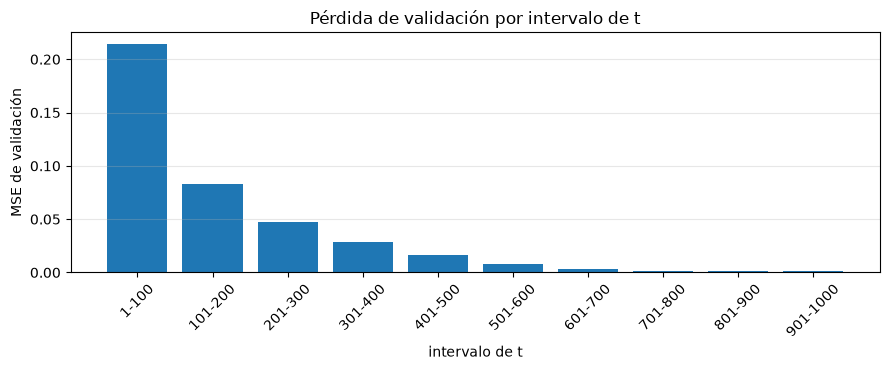
\includegraphics[width=0.85\textwidth]{figs/diff_loss_int.png}
\caption{Pérdida de validación (5\,000 imágenes) por intervalo de $t$ de 100 pasos.}
\end{figure}

\subsection*{Task 3.3 --- Muestreo ancestral}
\[x_{t-1}=\frac1{\sqrt{\alpha_t}}\Big(x_t-\frac{1-\alpha_t}{\sqrt{1-\bar\alpha_t}}\hat\epsilon\Big)+\sigma_t z,\quad \sigma_t^2=\beta_t,\ z=0\text{ en el último paso}\]

\begin{figure}[H]
\centering
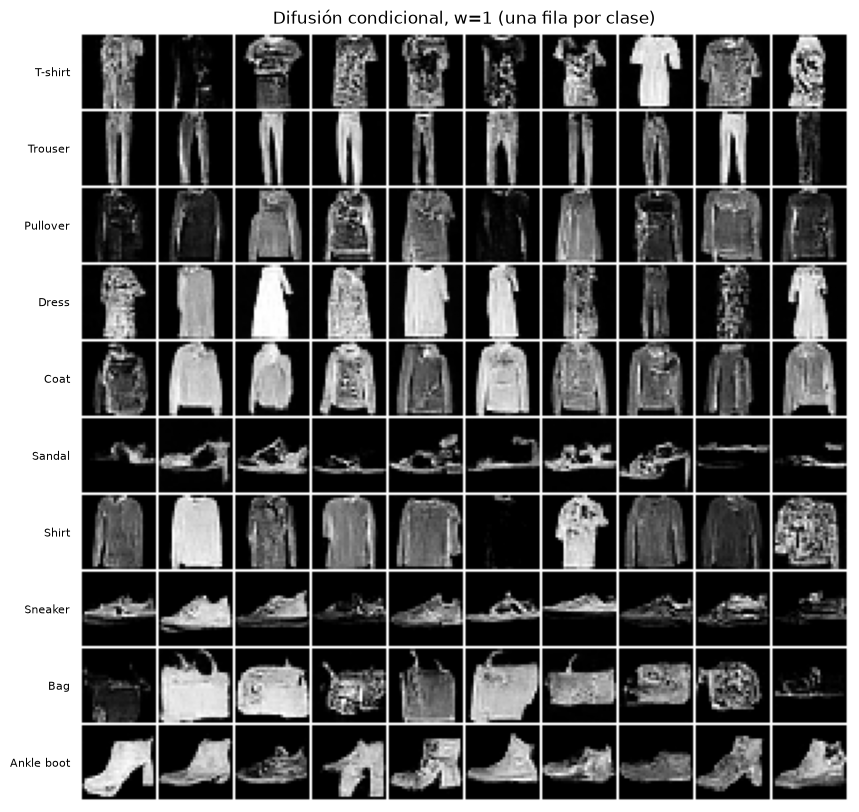
\includegraphics[width=0.7\textwidth]{figs/diff_samples_w1.png}
\caption{10 imágenes por clase con $w=1$, una fila por clase.}
\end{figure}

\subsection*{Task 3.4 --- Guía sin clasificador}
\textbf{(a)} Predicción guiada, con $w=1$ equivalente al modelo condicional puro:
\[\tilde\epsilon=\epsilon_\theta(x_t,t,\varnothing)+w\,(\epsilon_\theta(x_t,t,c)-\epsilon_\theta(x_t,t,\varnothing))\]

\textbf{(b--c)} 50 imágenes por clase para cada $w\in\{1,3,7\}$. Clasificador sencillo entrenado sobre imágenes reales hasta $\geq$ 88\% de exactitud en validación (exactitud obtenida: 0.8874). Diversidad = distancia euclidiana media entre pares de imágenes generadas de la misma clase (promediada sobre clases); referencia con 50 imágenes reales por clase.

\textbf{(d)}
\begin{table}[H]
\centering
\begin{tabular}{cccc}
\toprule
$w$ & fidelidad & diversidad & s / 100 imgs \\
\midrule
1 & 0.784 & 7.937 & 2.807 \\
3 & 0.952 & 7.880 & 6.831 \\
7 & 0.878 & 7.592 & 6.133 \\
\bottomrule
\end{tabular}
\end{table}
Diversidad de referencia (real, 50/clase): 8.838.

\begin{figure}[H]
\centering
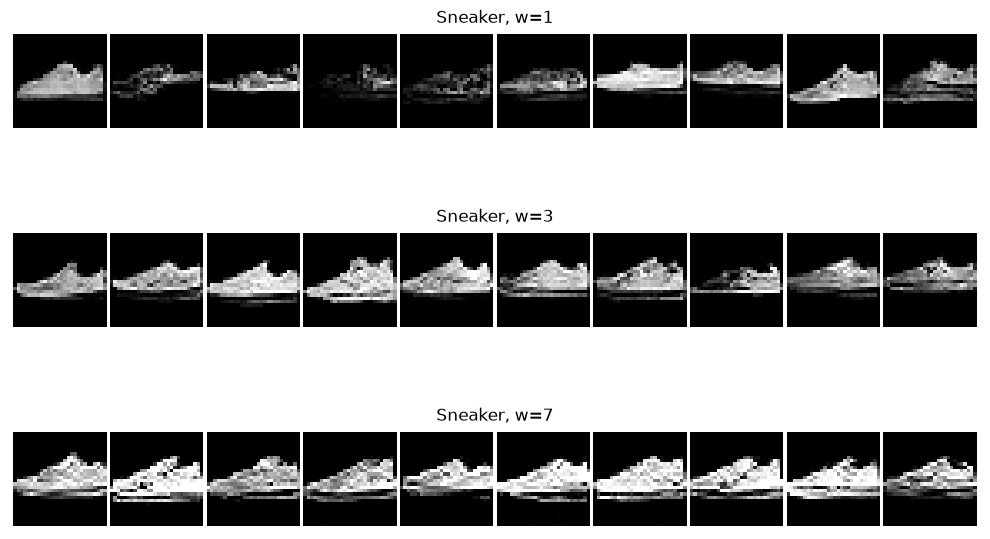
\includegraphics[width=0.85\textwidth]{figs/cfg_sneaker.png}
\caption{10 muestras de Sneaker para cada $w$.}
\end{figure}

\subsection*{Task 3.5 --- Análisis}

\subsubsection*{(a) Cambio de fidelidad y diversidad con $w$; clase cuya diversidad más cae entre $w=1$ y $w=7$}
\begin{table}[H]
\centering
\begin{tabular}{lccccc}
\toprule
Clase & real & $w=1$ & $w=3$ & $w=7$ & caída $w1\rightarrow w7$ (\%) \\
\midrule
T-shirt & 9.371 & 7.623 & 9.735 & 11.727 & $-53.8$ \\
Trouser & 7.235 & 6.412 & 5.440 & 5.095 & 20.5 \\
Pullover & 9.279 & 7.037 & 7.018 & 6.666 & 5.3 \\
Dress & 8.056 & 8.591 & 7.805 & 8.806 & $-2.5$ \\
Coat & 8.448 & 8.771 & 6.548 & 5.175 & 41.0 \\
Sandal & 9.458 & 6.909 & 8.641 & 12.377 & $-79.2$ \\
Shirt & 9.997 & 9.403 & 9.740 & 6.961 & 26.0 \\
Sneaker & 6.372 & 6.066 & 6.021 & 6.707 & $-10.6$ \\
Bag & 11.320 & 10.575 & 10.599 & 5.208 & 50.8 \\
Ankle boot & 8.839 & 7.988 & 7.251 & 7.197 & 9.9 \\
\bottomrule
\end{tabular}
\end{table}

\begin{table}[H]
\centering
\begin{tabular}{cccc}
\toprule
$w$ & fidelidad & diversidad & s / 100 imgs \\
\midrule
1 & 0.784 & 7.937 & 2.8 \\
3 & 0.952 & 7.880 & 6.8 \\
7 & 0.878 & 7.592 & 6.1 \\
\bottomrule
\end{tabular}
\end{table}

(Diversidad de referencia con 50 imágenes reales por clase: 8.838.)

\textbf{Tendencia.} La fidelidad sube de 0.784 a 0.952 al pasar de $w=1$ a $w=3$ (+17 puntos), pero baja a 0.878 con $w=7$: pasarse de guía deja de ayudar. La diversidad media cae de forma monótona (7.937 $\rightarrow$ 7.880 $\rightarrow$ 7.592, $-4.3\%$ de $w=1$ a $w=7$) y ya con $w=1$ queda por debajo de la real (8.838). Además, $w\neq1$ duplica el batch de la red en cada paso, por eso el tiempo pasa de 2.8 a 6--7 s por 100 imágenes.

\textbf{Clase más afectada: Bag}, cuya diversidad cae de 10.575 ($w=1$) a 5.208 ($w=7$), $-50.8\%$. Le siguen Coat (8.771 $\rightarrow$ 5.175, $-41.0\%$), Shirt ($-26.0\%$) y Trouser ($-20.5\%$).

\textbf{Hipótesis (respaldada por los datos).} Bag es la clase con mayor diversidad real (11.320, la más alta de las 10): sus imágenes varían muchísimo (formas, asas, patrones), así que tiene más diversidad que perder. La guía empuja hacia lo que el modelo considera más típico de la clase; en una clase tan heterogénea eso colapsa a unos pocos prototipos (la bolsa rectangular clara), y por eso cae más.

\textbf{Matiz sobre la métrica.} Algunas clases suben (T-shirt +54\%, Sandal +79\%, Sneaker +11\%). Con $w=7$ las imágenes salen saturadas y de mayor contraste, y la distancia euclidiana en píxeles crece con la intensidad, así que la métrica puede subir aunque la variedad de formas baje. Sneaker es el caso más claro: en la figura, con $w=7$ las 10 muestras son casi la misma zapatilla de alto contraste, pero su diversidad medida sube de 6.066 a 6.707. Es una limitación de usar distancia en píxeles como medida de diversidad.

\subsubsection*{(b) Matriz de confusión del clasificador sobre las imágenes generadas con $w=1$}
\begin{figure}[H]
\centering
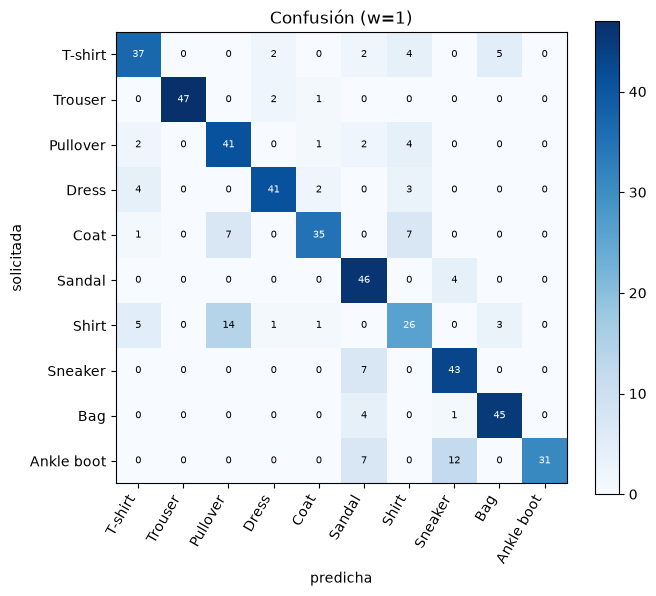
\includegraphics[width=0.6\textwidth]{figs/confusion.png}
\end{figure}
\begin{figure}[H]
\centering
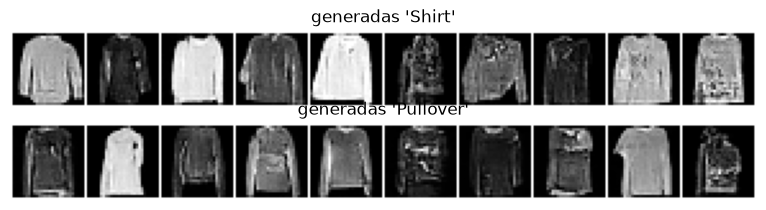
\includegraphics[width=0.85\textwidth]{figs/confusion_1.png}
\caption{Muestras generadas de Shirt (arriba) y Pullover (abajo), $w=1$.}
\end{figure}

La exactitud global con $w=1$ es $392/500=0.784$ (suma de la diagonal). El par más confundido es \textbf{Shirt $\rightarrow$ Pullover} (14 de 50 imágenes pedidas como Shirt). Shirt es además la clase peor lograda: solo 26/50 (52\%) se clasifican como Shirt. Le siguen Ankle boot $\rightarrow$ Sneaker (12), y con 7 cada una: Coat $\rightarrow$ Pullover, Coat $\rightarrow$ Shirt, Sneaker $\rightarrow$ Sandal y Ankle boot $\rightarrow$ Sandal.

\textbf{¿Defecto del generador, del clasificador o de las clases?} Principalmente de las propias clases, con una contribución del generador:
\begin{itemize}
  \item \textbf{Clases:} Shirt, Pullover, Coat y T-shirt son prendas de torso con manga larga muy parecidas. En las imágenes, las filas generadas de Shirt y Pullover son casi indistinguibles (mangas largas, cuerpo oscuro con textura), y lo mismo pasa con Ankle boot y Sneaker (calzado de perfil similar). Las confusiones ocurren justo entre grupos visualmente parecidos.
  \item \textbf{Generador:} con $w=1$ varias muestras salen ruidosas, de bajo contraste o con textura rara (se ve en la cuadrícula de la Task 3.3, p.\ ej.\ las filas de T-shirt y Dress), y esas muestras ambiguas son las que el clasificador confunde. La fidelidad sube a 0.952 con $w=3$, es decir, parte del error es del condicionamiento débil de $w=1$.
  \item \textbf{Clasificador:} su exactitud en validación es 0.8874, apenas sobre el 88\% pedido, así que también se equivoca. No calculé su matriz de confusión sobre datos reales; para confirmar que sus errores caen en los mismos pares habría que hacerlo.
\end{itemize}

\subsubsection*{(c) La guía corresponde a muestrear $\tilde p(x|c)\propto p(x)p(c|x)^w$}
\emph{Demostración.} Con $s(x_t\mid c)\approx-\epsilon_\theta(x_t,t,c)/\sqrt{1-\bar\alpha_t}$ y $s(x_t)\approx-\epsilon_\theta(x_t,t,\varnothing)/\sqrt{1-\bar\alpha_t}$, la predicción guiada $\tilde\epsilon=\epsilon_\varnothing+w(\epsilon_c-\epsilon_\varnothing)$ corresponde al score
\[\tilde s=s_\varnothing+w\,(s_c-s_\varnothing)=\nabla\log p(x)+w\left[\nabla\log p(x\mid c)-\nabla\log p(x)\right].\]
Por la regla de Bayes, $p(x\mid c)=p(c\mid x)p(x)/p(c)$, y como $p(c)$ no depende de $x$, al tomar el gradiente del logaritmo:
\[\nabla\log p(x\mid c)-\nabla\log p(x)=\nabla\log p(c\mid x).\]
Entonces
\[\tilde s=\nabla\log p(x)+w\,\nabla\log p(c\mid x)=\nabla\log\!\left[p(x)\,p(c\mid x)^w\right],\]
es decir, se muestrea de $\tilde p(x\mid c)\propto p(x)\,p(c\mid x)^w$. Para $w=1$ es $p(x)p(c|x)\propto p(x|c)$ (el modelo condicional puro), y para $w=0$ es $p(x)$ (incondicional).

\emph{Efecto sobre la diversidad.} Elevar $p(c\mid x)$ a $w>1$ amplifica las diferencias: las imágenes donde la clase es muy clara pesan mucho más y las ambiguas casi desaparecen (algo parecido a bajar la temperatura). La masa se concentra en pocos modos típicos de la clase y la diversidad baja. Es lo que se ve en los datos: diversidad 7.937 $\rightarrow$ 7.880 $\rightarrow$ 7.592 para $w=1,3,7$, con la caída más fuerte en Bag ($-50.8\%$). La fidelidad sube primero (0.784 $\rightarrow$ 0.952), pero con $w=7$ baja a 0.878: un factor tan grande lleva a pasos fuera de la distribución de datos y a imágenes saturadas.

\subsubsection*{(d) Intervalo de $t$ con mayor y menor pérdida y relación con el SNR}
MSE de validación por intervalo de $t$:
\begin{table}[H]
\centering
\begin{tabular}{lccccc}
\toprule
intervalo & 1--100 & 101--200 & 201--300 & 301--400 & 401--500 \\
MSE & 0.2145 & 0.0826 & 0.0478 & 0.0287 & 0.0162 \\
\midrule
intervalo & 501--600 & 601--700 & 701--800 & 801--900 & 901--1000 \\
MSE & 0.0080 & 0.0036 & 0.0017 & 0.0011 & 0.0010 \\
\bottomrule
\end{tabular}
\end{table}

La pérdida es \textbf{mayor en el intervalo 1--100 (0.2145)} y \textbf{menor en el 901--1000 (0.0010)}, unas 215 veces menor, y decrece de forma monótona. Los dos primeros intervalos concentran el 73\% de la suma de las pérdidas.

\textbf{Relación con el SNR (Task 2.5b).} Con SNR alto ($t$ pequeño) $x_t\approx x_0$ y el ruido es una perturbación mínima que la red solo puede separar si reconoce el detalle fino de la imagen: la tarea es la más difícil. En el calendario lineal, los primeros $\sim$27 pasos tienen SNR $>100$ y el SNR cruza 1 en $t=260$. Con SNR bajo, $x_t\approx\epsilon$ y predecir $\epsilon$ se reduce a copiar $x_t$ (reescalado): en el calendario lineal los 326 pasos con SNR $<0.01$ ($t\ge675$) cubren los intervalos 701--1000 y el final del 601--700, donde la pérdida es $\le0.0036$.

\textbf{¿Coincide con lo que predije?} Sí. En 2.5(b) anticipé que los pasos de SNR muy alto serían los más difíciles y los de SNR muy bajo casi triviales, y la gráfica lo confirma. Además, estos últimos aportan muy poco gradiente cuando $t$ se sortea uniformemente, lo que explica por qué el calendario propio (coseno), con 880 pasos en el rango informativo contra 647, es más eficiente.

% =====================================================================
\section*{Task 4 --- Comparación de familias y pass@k}

\subsection*{Task 4.1 --- VAE vs.\ difusión}

\subsubsection*{(a) Nitidez sobre 500 imágenes de cada fuente}
\begin{table}[H]
\centering
\begin{tabular}{lcc}
\toprule
 & nitidez & \% de la real \\
\midrule
Real & 0.0886 & 100\% \\
Difusión ($w=1$) & 0.0739 & 83\% \\
VAE ($\beta=1$) & 0.0508 & 57\% \\
\bottomrule
\end{tabular}
\end{table}

\subsubsection*{(b) Tiempo de generación de 100 imágenes y evaluaciones de red}
\begin{table}[H]
\centering
\begin{tabular}{lcc}
\toprule
 & tiempo (100 imgs) & evaluaciones de red \\
\midrule
VAE ($\beta=1$) & 0.3 ms & 1 \\
Difusión ($w=1$) & 1785.6 ms & 1000 \\
\bottomrule
\end{tabular}
\end{table}
Razón de tiempos difusión / VAE $\approx$ \textbf{6341$\times$}.

\subsubsection*{(c) Mapa de compensaciones y cómo acortar la difusión}
\begin{itemize}
  \item \textbf{VAE:} rápido (una pasada del decoder) y estable (pérdida determinista, sin adversario), pero borroso: con MSE el decoder predice $\mathbb E[x\mid z]$ y promedia los bordes (Task 1.4d).
  \item \textbf{Difusión:} más nítida (83\% vs.\ 57\% de la nitidez real) y también estable (un MSE sencillo), pero $\sim$6300$\times$ más lenta por sus $T=1000$ evaluaciones secuenciales.
\end{itemize}

Ambas ganan en estabilidad; la compensación real es \textbf{nitidez vs.\ velocidad}.

\textbf{Para acortar la difusión:} muestrear con menos pasos (p.\ ej.\ DDIM con $\sim$50 pasos, $\sim$20$\times$ menos evaluaciones), destilar el modelo a pocos pasos (destilación progresiva o modelos de consistencia) o usar una U-Net más pequeña. Además, evitar $w\neq1$, que duplica el batch y multiplica el costo por $\sim$2.4 (6.8 vs.\ 2.8 s / 100 imgs).

\subsection*{Task 4.2 --- pass@k}

\subsubsection*{(a) pass@1, pass@5 y pass@10 con el estimador insesgado}
\begin{table}[H]
\centering
\begin{tabular}{lccc}
\toprule
 & pass@1 & pass@5 & pass@10 \\
\midrule
P1 & 0.0000 & 0.0000 & 0.0000 \\
P2 & 0.1000 & 0.4474 & 0.7632 \\
P3 & 0.2500 & 0.8063 & 0.9837 \\
P4 & 0.4500 & 0.9702 & 0.9999 \\
P5 & 0.7000 & 0.9996 & 1.0000 \\
P6 & 1.0000 & 1.0000 & 1.0000 \\
\midrule
\textbf{promedio} & \textbf{0.4167} & \textbf{0.7039} & \textbf{0.7911} \\
\bottomrule
\end{tabular}
\end{table}

\textbf{P2, $k=5$} ($n=20$, $c=2$, $n-c=18\ge5$):
\[\text{pass@5}=1-\frac{\binom{18}{5}}{\binom{20}{5}}=1-\frac{8568}{15504}=1-0.5526=\mathbf{0.4474}.\]

\subsubsection*{(b) P2: $\text{pass@}k=1-\frac{(20-k)(19-k)}{380}$ y menor $k$ con pass@$k>0.9$}
\emph{Demostración.} Para $n=20$, $c=2$:
\[\frac{\binom{18}{k}}{\binom{20}{k}}=\frac{18!}{k!\,(18-k)!}\cdot\frac{k!\,(20-k)!}{20!}=\frac{(20-k)(19-k)}{20\cdot19}=\frac{(20-k)(19-k)}{380}\]
\[\Rightarrow\ \text{pass@}k=1-\frac{(20-k)(19-k)}{380}.\]
La celda verifica que coincide con el estimador para $k=1,\dots,20$.

\emph{Menor $k$:} $k=13$ da $1-\frac{42}{380}=0.8895$ y $k=14$ da $1-\frac{30}{380}=0.9211$, así que $\mathbf{k=14}$.

\subsubsection*{(c) Estimador insesgado vs.\ ingenuo, $k=5$}
\begin{table}[H]
\centering
\begin{tabular}{lccc}
\toprule
 & insesgado & ingenuo & diferencia \\
\midrule
P1 & 0.0000 & 0.0000 & 0.0000 \\
P2 & 0.4474 & 0.4095 & 0.0379 \\
P3 & 0.8063 & 0.7627 & 0.0436 \\
P4 & 0.9702 & 0.9497 & 0.0205 \\
P5 & 0.9996 & 0.9976 & 0.0020 \\
P6 & 1.0000 & 1.0000 & 0.0000 \\
\bottomrule
\end{tabular}
\end{table}

El ingenuo nunca supera al insesgado; la brecha es mayor en los problemas intermedios (P2, P3) y nula en los extremos (P1, P6).

\emph{Demostración.} Si $n-c<k$, el insesgado vale 1 $\ge$ ingenuo. Si $n-c\ge k$:
\[\frac{\binom{n-c}{k}}{\binom nk}=\prod_{i=0}^{k-1}\frac{n-c-i}{n-i}\le\left(\frac{n-c}{n}\right)^k=\left(1-\frac cn\right)^k,\]
y restando de 1 se invierte la desigualdad: ingenuo $\le$ insesgado.

\emph{Intuición.} El ingenuo muestrea con reemplazo; el insesgado, sin reemplazo, no repite soluciones fallidas y por eso es más probable que encuentre una correcta.

\subsubsection*{(d) Agente que reintenta hasta 10 veces con verificador perfecto}
Con hasta 10 intentos y un verificador perfecto, el agente resuelve \textbf{P2--P6} (todos con $c>0$), con probabilidad pass@10: 0.76 en P2, 0.98 en P3 y $\ge0.9999$ en P4--P6. \textbf{P1} ($c=0$) no se resuelve nunca.

El promedio sube de \textbf{0.417} (pass@1) a \textbf{0.791} (pass@10), casi el doble: el modelo sabe resolver la mayoría de los problemas, pero no de forma consistente, y reintentar con verificación compensa esa inconsistencia. El techo es $5/6\approx0.833$ (fracción con $c>0$); lo que falta (P1) requiere un mejor modelo, no más intentos.

\newpage

\printbibliography

\end{document}
